\documentclass[letterpaper,12pt]{article}
\usepackage{booktabs,graphicx,amssymb,lineno,amsmath,multirow,rotating,verbatim,setspace,float,subfigure, fixltx2e}
\usepackage[margin=1in]{geometry}
\usepackage{gensymb}
\usepackage[table]{xcolor}

%*******************************************************************************************************
% verbatim lets you do \begin{} and \end {} comment
%amsymb & amssymb useful for math.  
% check out the wiki page 
%/cite  or citep (with natbib package?)
%/textit or 

%added fixlt2e 

% Latex once to get the file
% Then bibtex (Put in the same WD)
% then typeset LaTex again by pushing typeset twice to get the citations in 

\begin{document}

\linenumbers
%\renewcommand{\thesubfigure}{\Alph{subfigure}}
%\bibpunct{[}{]}{,}{n}{,}{,}

\title{Summary of BTB-brucellosis coinfection model and assumptions}
\date{23-April-2016}

\maketitle
%\singlespace
\doublespacing

\section*{Overview}
Bovine tuberculosis (bTB) and brucellosis are positively associated at the population level.   Age prevalence curves show a shift in the peak age of brucellosis infection in co-infected animals (Figure 1).  We want to know why, so we investigate the costs of co-infection on three parameters relevant for disease dynamics. \\
1. \textit{Host mortality rates}: bTB was associated with a 2.81 ($95\% CI 1.47-6.82$) fold increase in mortality hazard and infection with brucellosis was associated with an 3.00 ($95\% CI 1.50-6.01$) fold increase in mortality hazard compared to uninfected buffalo.  We did not find support for an interaction between bTB and brucellosis on mortality, indicating that the mortality effects of both infections are additive in co-infected buffalo.   \\
2. \textit{Incidence rates}:  bTB was associated with a 1.37 fold increase in the rate at which animals acquire brucellosis.   This pattern occurred in one site but not the second.  I think this is because the higher baseline mortality in the second site means we do not catch and diagnose infected individuals before they die and hope to test this with the model.\\
3. \textit{Pregnancy rates}:  These analyses are still in prep- in general we see declines with infection \\
The model then asks, (1) are changes in these rates sufficient to generate the age prevalence patterns observed and (2) what is the consequence of co-infection for disease invasion?


\begin{figure}
\begin{center}
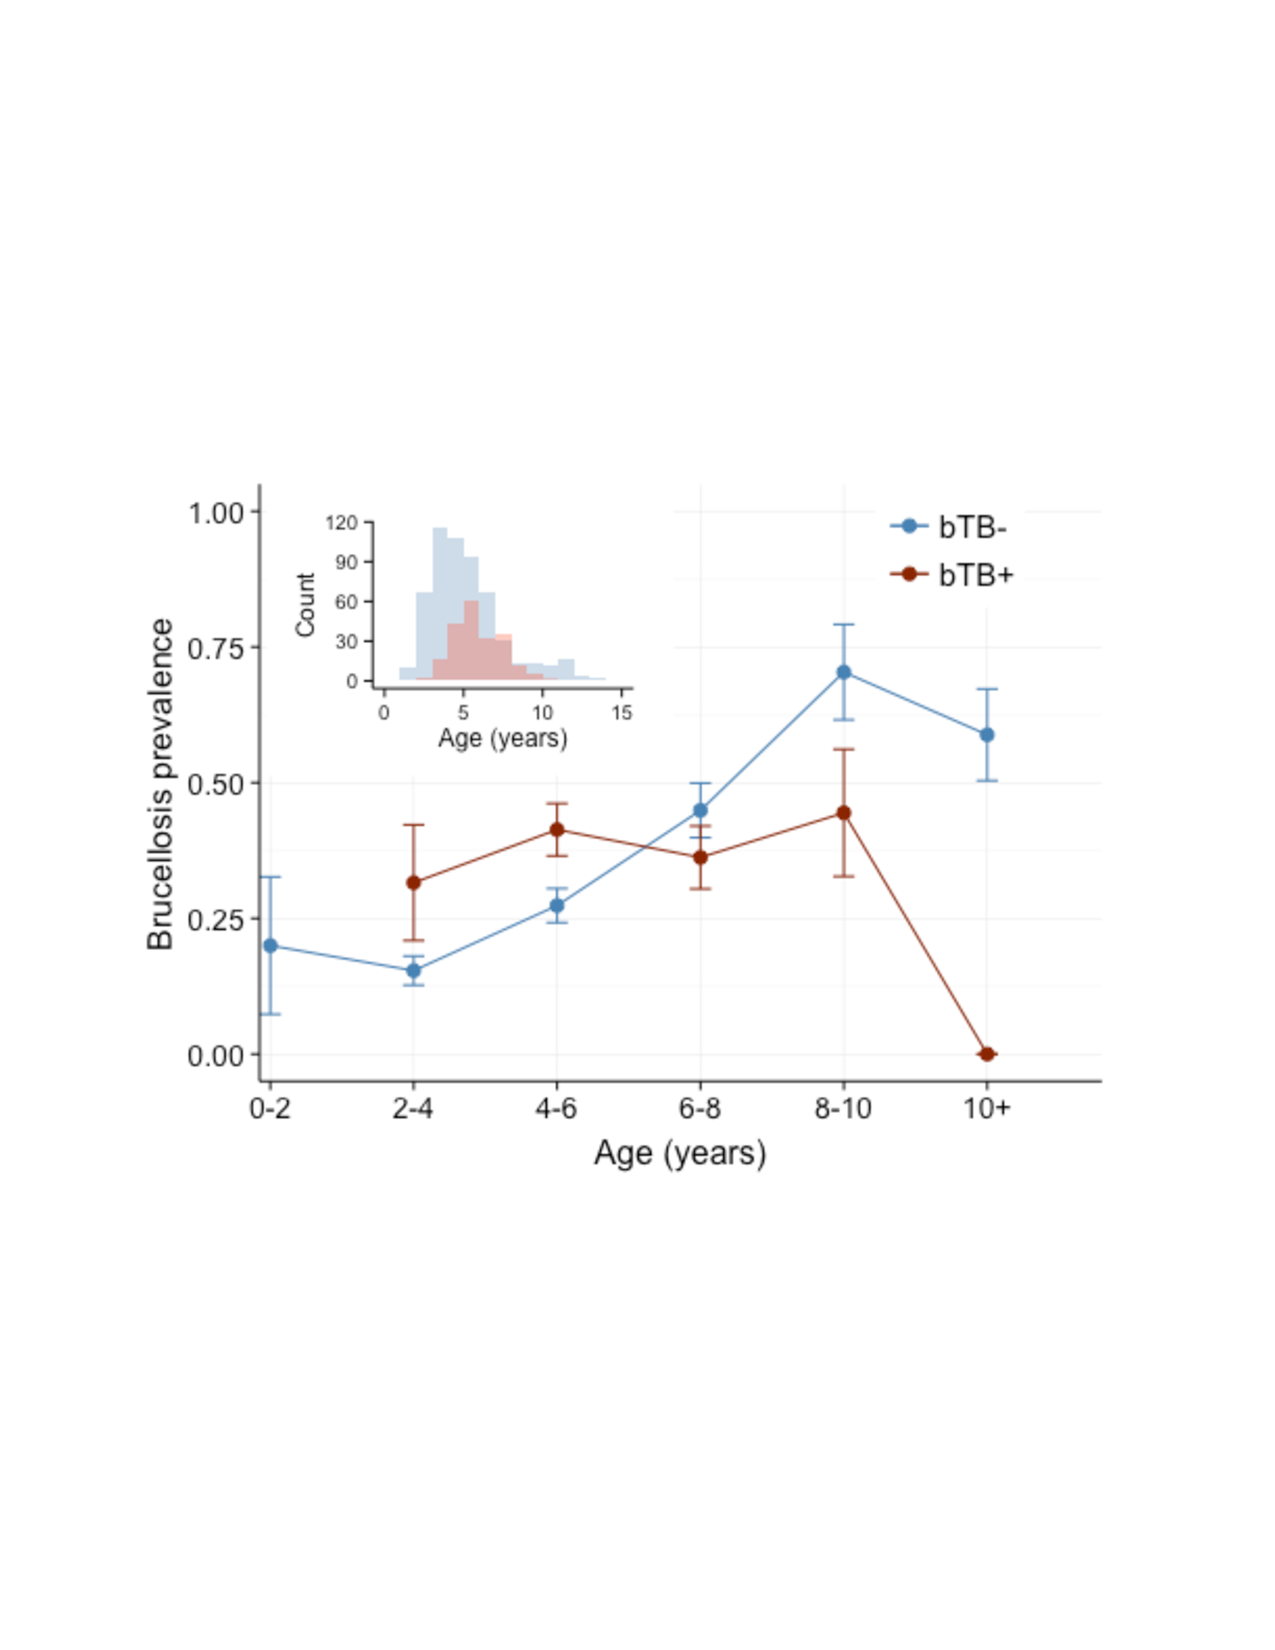
\includegraphics[width=5in]{Figure1_ageprev}
\end{center}
\caption{Age, brucellosis-prevalence curves in buffalo simultaneously uninfected (blue) or infected (red) with bTB.  The inset figure shows the distribution of ages in our sample, which best cover buffalo between two and eight years old and include 796 samples from 151 repeatedly captured individuals.  Ages are binned for visualization and animals that test positive are assumed to remain positive for the duration of the study.  Sample sizes for TB- are: 10, 182, 209, 103, 27, 35 buffalo.  Sample sizes for TB+ animals are: 0, 21, 108, 75, 21, 1 for ages 0-2, 2-4, 4-6, 6-8, 8-10, and 10+ respectively.}
\label{fig1}
\end{figure}

%%%%%%%%NOTE%%%%%%%%%%
% Think about last data point.
% Maybe remove 10+ TB positive point, put large CI on it. 

\pagebreak
\section*{Model Structure and Assumptions}

\indent
	We developed a continuous time differential equation model to evaluate the disease dynamic consequence of bTB invasion on brucellosis dynamics and vice versa.  
Our model structure reflects the costs of co-infection identified for each parameter: host mortality rate, host birth rate, and disease transmission rates (Figure 2).
Animals are represented with six groups: susceptible to both infections($S$), acutely infected with brucellosis ($I_B$), chronically infected with brucellosis ($C_B$), infected with bTB ($I_T$), co-infected with both pathogens ($I_C$), or in the chronic stages of brucellosis and infected with bTB ($C_C$).\\
Our model is not spatially explicit.  Buffalo herds within the regions studied have fission-fusion behavior, where herds come together and fragment over time (Cross et al. 2005).  Dispersal between regions also occurs (Spaan, Masters thesis).  If data become available to parameterize aggregation patterns and movement rates between herds during birthing periods, it is possible to extend this framework in a spatially explicit context.  We represent regional differences in the underlying survival and fecundity rates observed in our statistical analyses by considering parameters for both the Lower Sabie and Crocodile Bridge region.
% Why called recovered with recrudescence vs. Latent? 
% Maybe need to highlight the framework more- We incorporate uncertainty associated with the effects of infection and co-infection on host survival and disease transmission by simulating infection dynamics directly from posterior estimates from our statistical models.   

\noindent
\textit{Brucellosis}\\
	We model the transmission of brucellosis by assuming the time course of infection in African buffalo is comparable with infection in cattle and bison (\textit{Bison bison}) and by following model structures developed in those systems (Treanor et al. 2010, Vaccine, Ebinger et al. 2011, Hobbs et al. 2015).  
Clinical signs of brucellosis infection in cattle and bison include abortions and decreased milk production (Olsen and Tatum, 2010; Samartino and Enright 1993; Rhyan et al. 1994).  
In natural populations of African buffalo, infection is also associated with declines in condition in the dry season and mortality independent of host condition (Gorsich et al. 2015).  (Note this is similar to Moose! Forbes et al. 1996, Experimental studies on Brucella abortus in moose, JWD). 

In bison, brucellosis is associated with lower calving rates following sero-conversion.  Calving rates were also overall lower in some age classes with brucellosis, although the effect was non-significant (age $<$ 4, uninfected 0.64 (95\% CI: 0.52?0.76); test posive: 0.81 (95\% CI: 0.73?0.89);  after sero-conversion 0.22 (95\% CI: 0.00?0.46) )

The survival and reproductive costs of infection in bison (Fuller et al.2007)
%Analyses in buffalo did not find evidence for change in fecundity throughout the course of brucellosis infection, so we assume this is also the case in African buffalo. 

"However, some animals may completely clear the bacterium and recover (John and Samuel 2000, Ficht 2003), while other animals appear have a natural resistance to the disease (Templeton et al. 1988, Derr et al. 2002)."


Transmission of brucellosis to susceptible bison or cattle occurs primarily through ingestion of  the bacteria shed in association with an aborted fetus, reproductive tissues or discharges during birthing (Samartino and Enright 1993).  The bacteria has been isolated from placental samples after brucella-induced abortions and milk (Alexander et al. 1981; Capparelli et al. 2009).    Thus, although males acquire infection, pregnant females are assumed to transmit the infection (seaman source).  In bison, risk of shedding the bacteria is highest 2 years after infection
After 2 years, xxxx abortions??? .

The incubation period ranges with age, sex, stage of gestation, and susceptibility (Nicoletti).


Based on the ranging behavior and size of buffalo herds (Ryan et al. 2007), we assume contact patterns are constant across a range of host densities and model transmission as frequency dependent.
Animals remain infected and infectious with brucellosis for two years following seroconversion (Rhyan et al. 2009).  
During this time, they suffer decreased birth and survival rates. 
Recovered animals are associated with similar pregnancy rates as uninfected buffalo and do not contribute to transmission. %?survival and pregnancy
A small percentage of recovered buffalo, $\eta$, can recrudesce and actively transmit the infection. (Note: this assumptions about time course of infection are why I am redoing my pregnancy analyses so is subject to change) \\
More on latency from Ray et al., 1988; Dolan et al. 1980. 
% to discussion- incidence moth didn't look too pulsed... so the continuous time assumption is maybe more ok than in more temperate climates with a more protracted birthing season.
We also represent the possibility of vertical transmission of brucellosis because bacteria have been detected in the placenta, fetal fluid, and colostrum of infected cattle and bison (cattle: Alexander et al. 1981; Emminger and Schalm 1943, bison: Davis et al. 1990, Xavier et al. 2009).
Experimental evidence from cattle suggests vertical transmission is infrequent (Fensterbank 1978; Plommet et al. 1973).  
Similarly, maternal immunity in bison calves wanes after 5-6 months and is no difference in the rate that calves borne to seronegative and seropositive mothers become infected (Fuller et al. 2007, Ryan et al. 2009).
Serological evidence suggests that vertical transmission is also rare in African buffalo (Gorsich et al. 2015).
Thus, we allow a small proportion of African buffalo calves, $\rho$, to acquire the infection. \\%but note that the importance of vertical transmission on the persistence of brucellosis in wildlife populations remains unclear.


\begin{figure}
\begin{center}
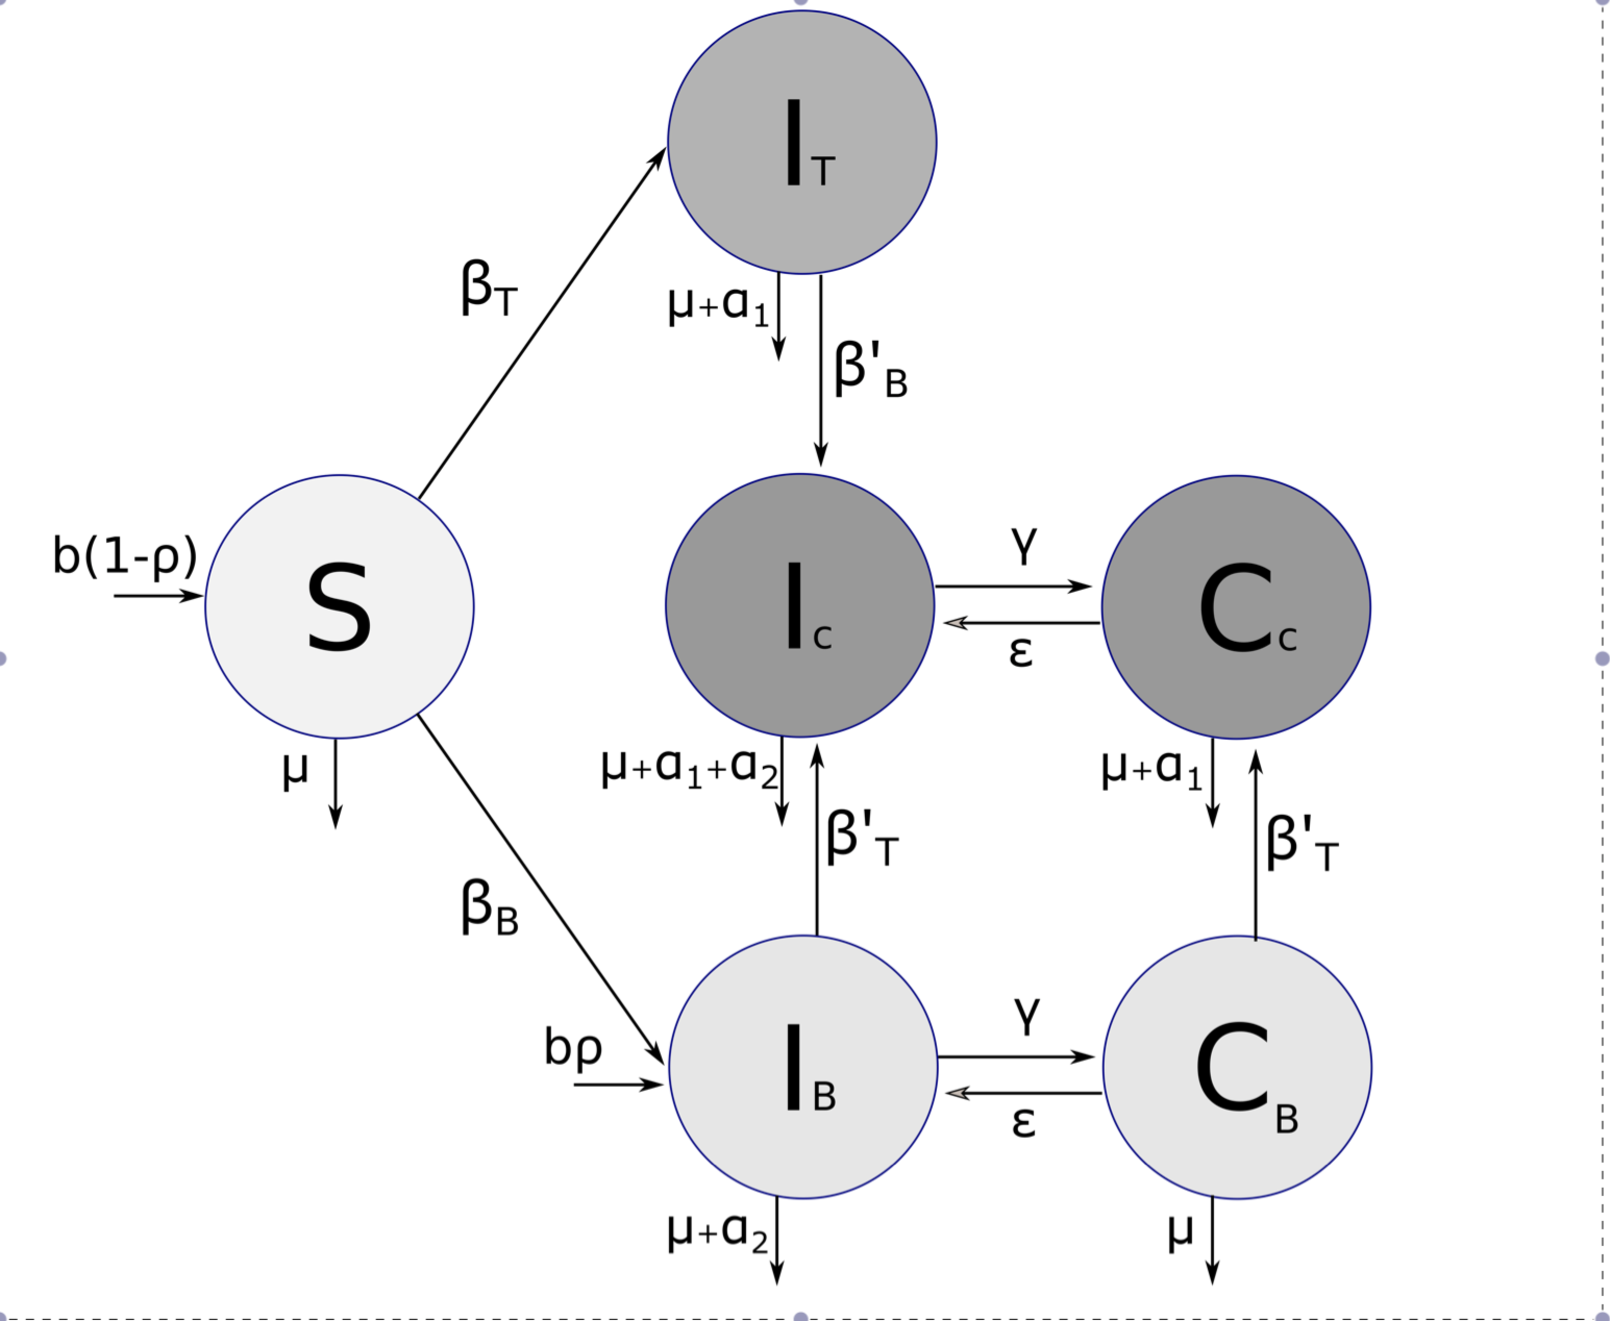
\includegraphics[width=4.5in]{Figure2_modelstructure}
\end{center}
\caption{Schematic representation of model structure}
\label{fig2}
\end{figure}

bTB infection in African buffalo is a lifelong infection (Bengis 1999) so we do not include a recovered class or clearance of the infection for bTB.  
Our assumptions about how bTB infection and co-infection with brucellosis effect survival, fecundity and transmission rates are detailed in the analyses section.  
% Something here about how we extrapolate the effect outside the age structures we sampled in our analyses. 
Together, the statistical results identified in this paper and these assumptions generate the following model: 
\begin{align*}%[hb]
N=& S+I_T+I_B+ I_C+ R_B + R_C \\
N_b=& S+b_1I_T+ b_2 I_B+ b_3 I_C + R_B + b_1 R_C
\end{align*}

\begin{align}
\frac{dS}{dt}&= b (1-\rho) N_b \left(1-\frac{r}{b}\frac{N}{K}\right)  - \beta_T S \frac{(I_T+I_C+ R_C)}{N} - \beta_B S \frac{(I_B+I_C)}{N} - \mu S\\
\frac{dI_T}{dt}&= \beta_T S \frac{(I_T+I_C+ R_C)}{N} -  \beta'_B I_T \frac{(I_B+I_C)}{N}  - (\mu+ \alpha_1) I_T \\
\frac{dI_B}{dt}&=  b \rho N_b \left(1-\frac{r}{b}\frac{N}{K}\right) + \beta_B S \frac{(I_B+I_C)}{N}  + \epsilon R_B - \gamma I_B - \beta'_T I_B \frac{(I_T+I_C+ R_C)}{N}- (\mu+ \alpha_2) I_B  \\
\frac{dI_C}{dt}&=  \beta'_T I_B \frac{(I_T+I_C+ R_C)}{N} +  \beta'_B I_T \frac{(I_B+I_C)}{N} + \epsilon R_C - \gamma I_C - (\mu+ \alpha_1 + \alpha_2) I_C \\
\frac{dR_B}{dt}&= \gamma I_B - \epsilon R_B - \mu R_B\\
\frac{dR_C}{dt}&=  \beta'_T R_B \frac{(I_T+I_C+ R_C)}{N} + \gamma I_C - \epsilon R_C - (\mu+ \alpha_1) R_C
\end{align}
where $N$ is the total host population and $r=b-\mu$ is the natural growth rate without density dependence.


%TB: "We found a significant regional variation in age structure, particularly in the 1-3 yr class, which may suggest a reduction in calf survival caused by a decrease in body condition of adult females and a subsequent decrease in milk production (Markusfeld et al. 1997, Hernandez and Baca 1998), Caron et al. 2003"


\section*{Approach}
Mortality and Fecundity parameters: \\
- Data analyses informs mortality rates for each disease category in \textit{young females aged 2-8)}.  \\
- Data analysis informs fecundity rates for each disease category in \textit{young females aged 2-8)}.  \\
- How to extrapolate to males and other age groups (Figure 3)?  \\
Parameters relevant to the time course of brucellosis are limited to cattle and U.S. bison: \\
- Pull $\gamma$ and $\epsilon$ from the literature.  \\
- Few animals were followed less than 2 years so assume our estimates are relevant for $I_B$.  Still thinking about this. \\
Transmission: \\
- Data analyses inform the proportional increase in transmission with co-infection (e.g. that $\beta'_B = 2.8 * \beta_B$).
 I hope to estimate $\beta_B$ and $\beta_T$ from the time sequence data.

\begin{figure}
\begin{center}
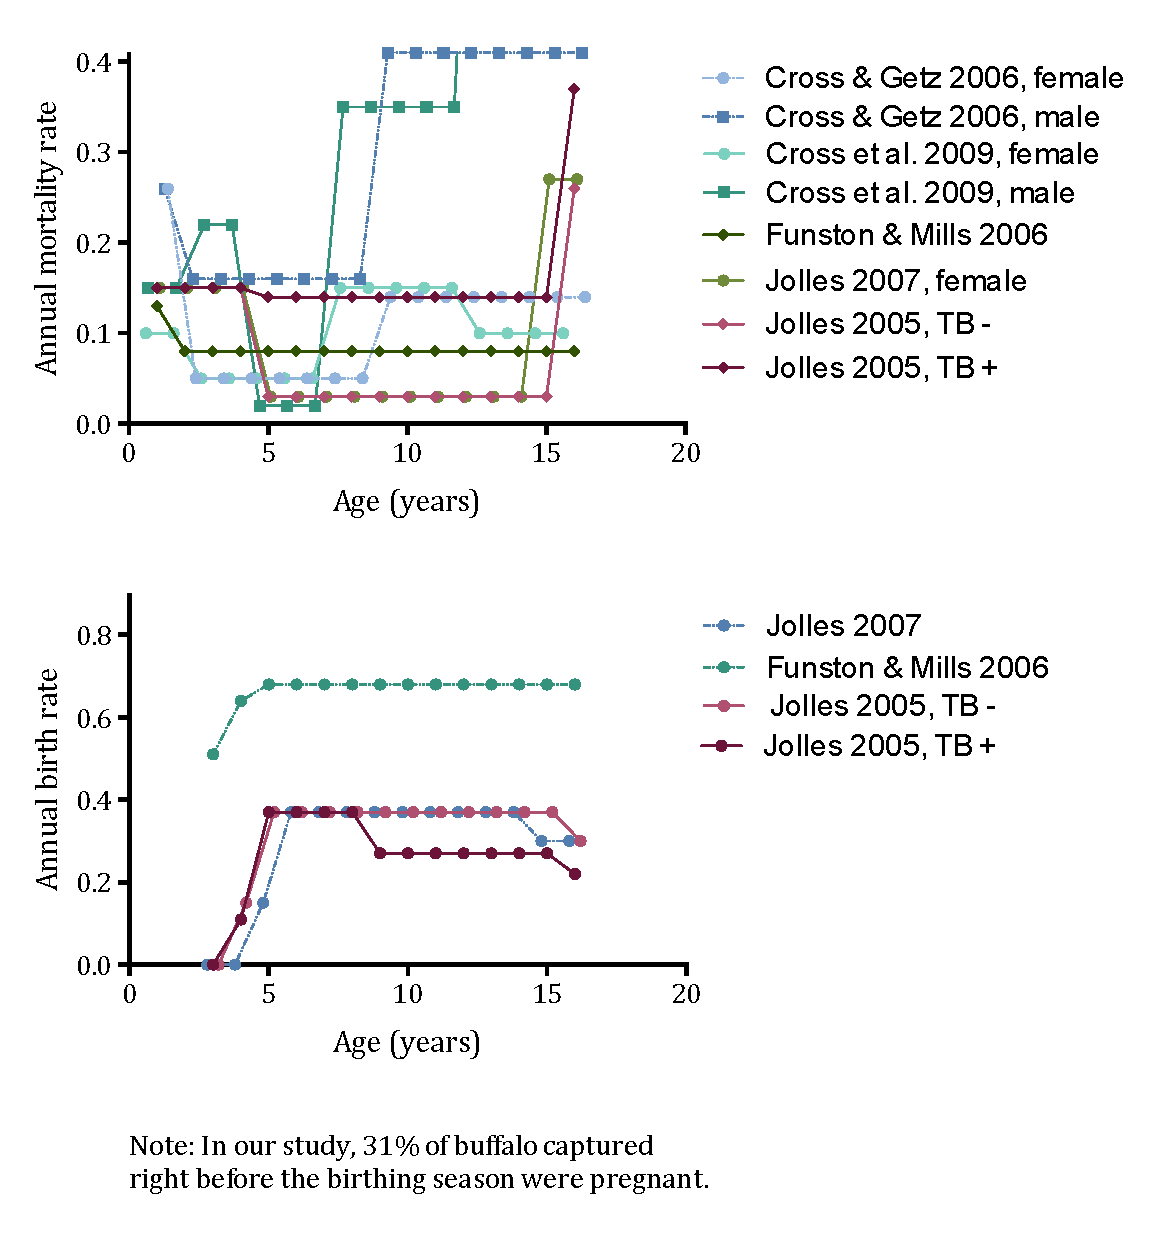
\includegraphics[width=5.5in]{Figure3_parametersummary}
\end{center}
\caption{Survival and fecundity parameters estimated on buffalo in South Africa}
\label{fig3}
\end{figure}

\begin{figure}
\begin{center}
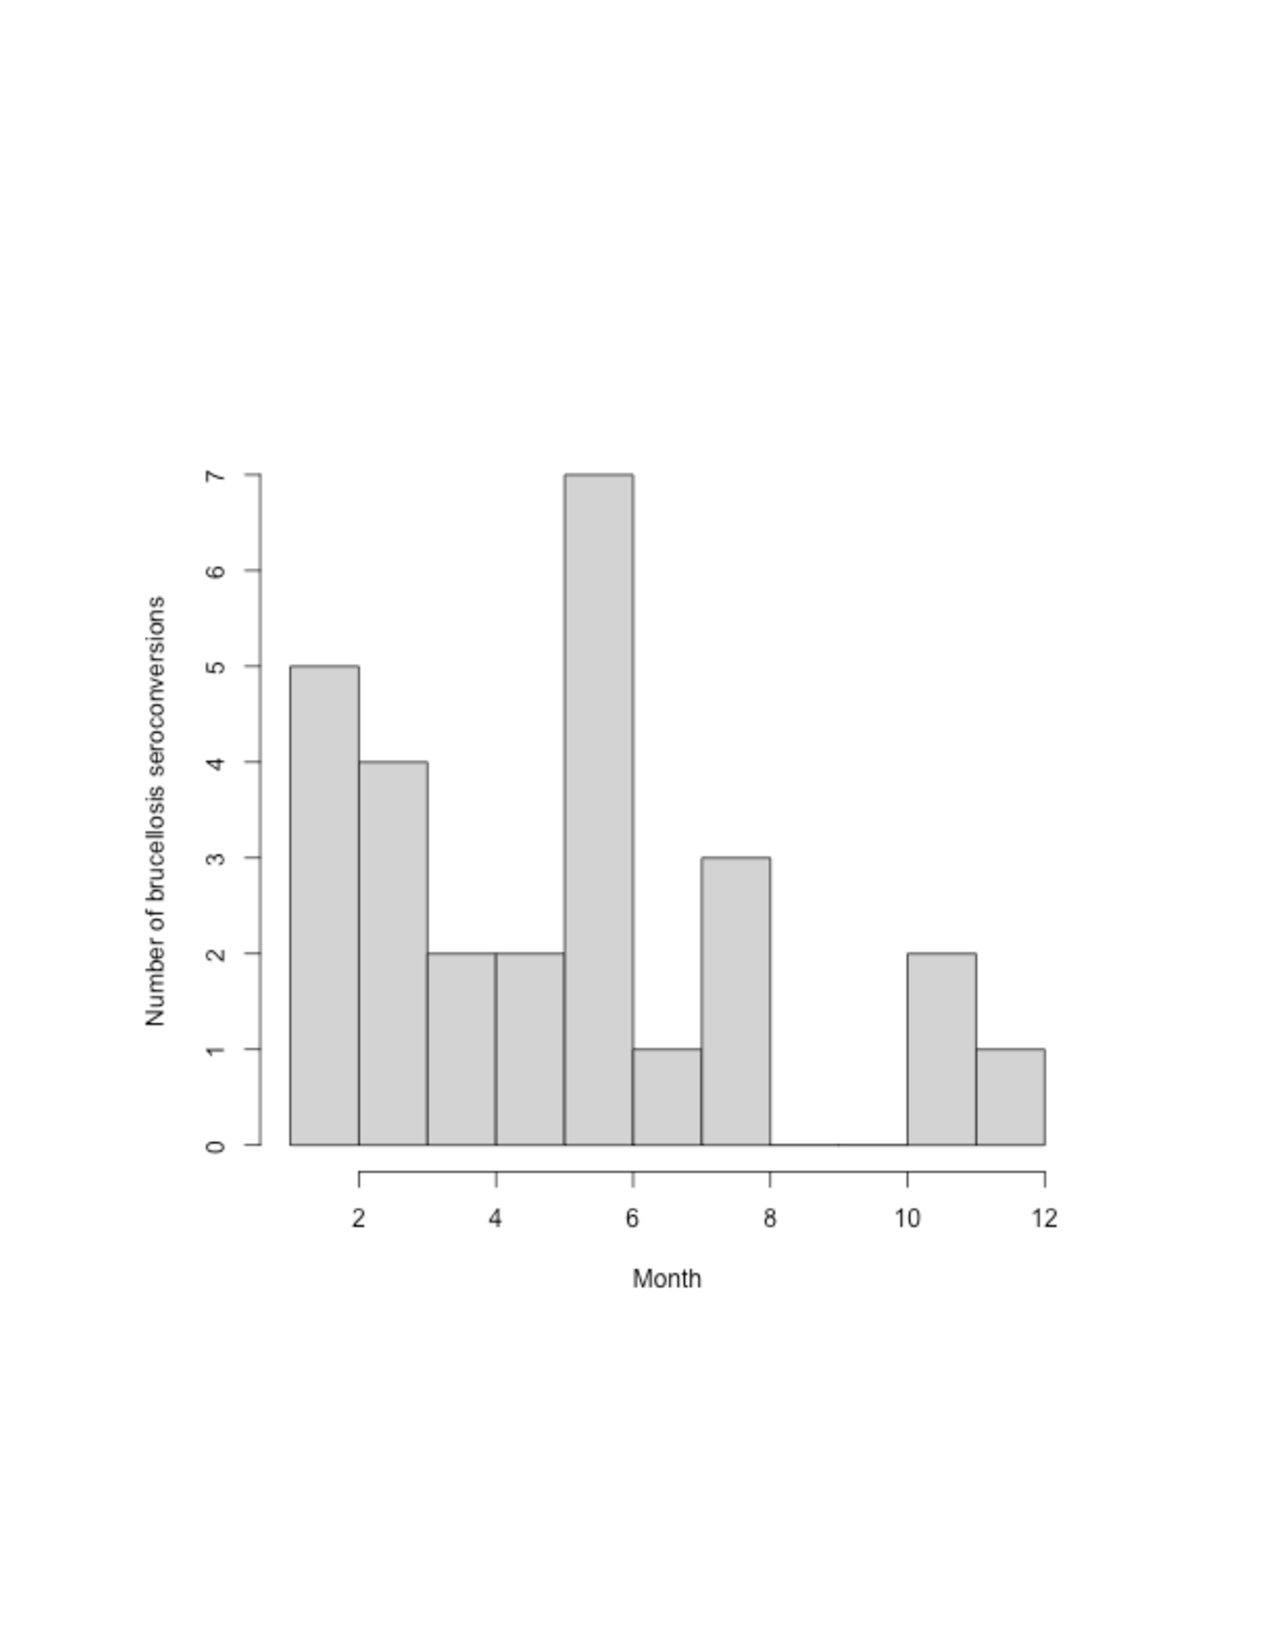
\includegraphics[width=5.5in]{Bruc_conversion_month}
\end{center}
\caption{Month when incidences occurred}
\label{fig4}
\end{figure}


%%%%%%%%%%%
% Try plotting relative mortality rates (males/females) to get a constant change. 
% And relative mortality rates for young/prime and old/prime to get a constant change
%then can extrapolate beyond age groups. 


\pagebreak


\textbf{Parameter table}
\begin{table}[hb]
\newcommand{\head}[1]{\textnormal{\textbf{#1}}}
\small
\begin{tabular}{lccp{12cm}}
\hline
\head{ } & \head{Value} & \head{Unit} & \head{Meaning}\\
\hline
b & $ figure $ & 1/d &  natural birth rate for uninfected animals \\
b1 & $?$ & 1/d & proportional reduction in birth rate for animals with bTB \\
b4 & $? $ & 1/d &proportional reduction in birth rate for animals with brucellosis.  \\
b5& $? $ & 1/d & proportional reduction in birth rate for co-infected animals.  \\

$\mu$& $0.067/365.25$& 1/d& natural death rate for uninfected animals.\\
K& $1000$& indiv & carrying capacity \\
 $\beta_T$& $0.0001/365.25$& 1/d& transmission rate for bTB \\
 $\beta_A$& $0.01/365.25$& 1/d& transmission rate for the acute infection \\
 $\beta_{T_A}$& $0.02/365.25$& 1/d& transmission rate for the acute infection for animals with bTB \\
 $\gamma_A$& $1/3$& 1/d& 1/duration of infection for acute pathogens \\
 $\gamma_{T_A}$& $1/3$& 1/d& 1/duration of infection for acute pathogens for individuals with bTB \\
 $\alpha_T$& $0.001/365.25$& 1/d& increase in the mortality rate due to bTB infection \\
  $\alpha_T$& $0.001/365.25$& 1/d& increase in the mortality rate due to bTB infection \\ 
 $\alpha_T$& $0.001/365.25$ & 1/d& increase in the mortality rate due to bTB infection \\
 r & b$-\mu$ & 1/d & population growth rate at small population sizes \\
\hline 
\end{tabular}
\end{table}
\\
\pagebreak






Let's consider first the TB-only model:
\begin{align}
\frac{dS}{dt}&=b N_b\left(1-\frac{r}{b}\frac{N}{K}\right) -\beta_T S I_T - \mu S\\
\frac{dI_T}{dt}&=\beta_T S I_T - \alpha_T I_T - \mu I_T
\end{align}

Then the disease free equilibrium is $E^0=(K,0)$ where the population is $x=(S,I_T)$. The basic reproduction number is $\mathcal{R}_0=\frac{\beta_T K}{\alpha_T + \mu}$. The endemic equilibrium is $E^*=(S^*,I_T^*)$ where $S^*=K\frac{1}{\mathcal{R}_0}$ and 
\begin{equation*}
I^*=K\left( \frac{r-\alpha_T}{2r}-\frac{1}{\mathcal{R}_0} + \frac{1}{2r}\sqrt{(r-\alpha_T)^2 + \frac{4r\alpha_T}{\mathcal{R}_0}}\right).
\end{equation*}
When $\alpha_T=0$, then $I^*=K(1-1/\mathcal{R}_0)$. We fix other parameters and vary $\beta_T$ to get endemic levels such that $I^*/N=10\%$, etc.
\pagebreak



\section*{Citations}

Alexander, B., Schnurrenberger, P.R., Brown, R.R. 1981. Numbers of Brucella abortus in the placenta, umbilicus and fetal fluid of two naturally infected cows. Veterinary Record. 108, 500. 

Begon et al. 2002. A clarification of transmission terms in host-microparasite models: numbers, densities and areas. Epidemiol. Infect. 129, 147-153.

Capparelli, R., Parlato, M., Iannaccone, M., Roperto, S., Marabelli, R., Roperto, F., Iannelli, D. 2009. Heterogeneous shedding of Brucella abortus in milk and its effect on the control of animal brucellosis. Journal of Applied Microbiology. 106, 2041-2047.

Cross et al. 2005. Disentangling association patterns in fission?fusion societies using African buffalo as an example. Animal Behaviour. 69, 499-506.

Davis et al. 1990. Brucella abortus in captive bison. I. Serology, bacteriology, pathogenesis, and transmission to cattle. 360-371.

Dolan, L.A. 1980. Latent carriers of brucellosis. 106, 241-243. 

Emminger, A.C., Schalm, O.W. 1943. The effect of Brucella abortus on the bovine udder and its secretion. Am.J. Vet. Res. 4, 100-109, 

Fensterbank, R. 1978. Congenital brucellosis in cattle associated with localization in a hygroma. Veterinary Record. 103, 283-284.

Fuller et al. 2007. Reproduction and survival of Yellowstone bison. JWD. 71, 2365-2372.

McCallum et al. 2001. How should pathogen transmission be modeled. Trends Ecol. Evol. 16, 295-300.

Olsen, S. and Tatum, F. 2010. Bovine Brucellosis.

Plommet et al. 1973. Annales de Recherches Veterinaires. 4, 419. %!!!

Ray, W.C., Brown, R.R., Stringfellow, D.A., Schnurrenberger, P.R., Scanlan, C.M., Swann, A.I. 1988. Bovine brucellosis: an investigation of latency in progeny of culture positive cows. JAVMA. 192, 182-186.

Rhyan, J.C. et al. 2009. Pathogenesis and epidemiology of Brucellosis in Yellowstone bison: Serologic and culture results from adult females and their progeny. J.WD. 45, 729-478.

Rhyan, J. C., W. J. Quinn, L. S. Stackhouse, J. J. Henderson, S. R. Ewalt, J. B. Payeur, M. Johnson, and M. Meagher. 1994. Abortion caused by Brucella abortus biovar 1 in a free- ranging bison (Bison bison) from Yellowstone National Park. Journal of Wildlife Diseases 30:445-446.

Samartino, L.E. and Enright, F.M. 1993. Pathogenesis of abortion of bovine brucellosis. 

Treanor et al. 2010. Vaccination strategies for managing brucellosis in Yellowstone bison. 28S, F64-F72.

Xavier et al. 2009. Pathological, Immunohistochemical, and Bacteriological study of tissues and milk of cows and fetuses experimentally infected with Brucella abortus. J. Comp. Path. 140, 149-157. 

\end{document}